\chapter{Technical Issues}\label{chapter:technicalissues}
This chapter covers some of the problems encountered when turning the model from Chapter \ref{chapter:model} into code. This will not be an exhaustive list of all the challenges but will focus on the more interesting problems and solutions. A look at the final software design is yet to come in Chapter \ref{chapter:softwaredesign} so this chapter will not make too many explicit references to the actual classes and methods used and instead try and focus more on the algorithms and frameworks used.

  \section{ABM frameworks}
    \paragraph{What is an ABM framework?}
    The first challenge was to create a software environment to run the simulation. 
    \paragraph{Why use an ABM framework? - Gilbert and Bankes paper}
    Gilbert and Bankes (\cite{Gilbert2002}) explain the advantages and
    disadvantages of using pre-existing libraries and frameworks for Agent-Based Models rather
    than ``rolling your own.'' Using pre-existing libraries frees a
    programmer up from re-implementing common
    algorithms. However, they also require a programmer to understand the
    language they are written in and to work with the built-in
    assumptions used by the original writers. Gilbert and Bankes state
    that agent-based modeling tools that match their ideal specifications
    do not yet exist but that there is a trend towards better
    tools becoming available. Fortunately a few years later Allen (\cite{Allan2009}) and Berryman (\cite{Berryman2008}) survey many ABM frameworks and suggest that NetLogo, MASON and Repast are useful frameworks. Personal communication with EngD student Ed Manley (\cite{Manley2012}) at UCL working on traffic simulations led me to look at the Repast framework. Therefore it seemed in 2012 with only a few months to complete this project but a good understanding of Java, using a pre-built framework would require less work than starting from the bottom and building a framework dedicated to the project.
    \subsection{ABM frameworks considered}
      \paragraph{Review of ABM frameworks - Allen and Berryman papers, hands}
      \subsubsection{Repast}
        \paragraph{descriptions of features/pros and cons of Repast}
        Open source
        Mailing list
        Documentation
        Examples from Repast City
        Java
        Random number generation
        Integrates nicely with Eclipse (so quick to get started)
        - slower than mason
        - less support for learning algorithms
      \subsubsection{NetLogo}
        \paragraph{descriptions of features/pros and cons of Netlogo}
        NetLogo requires the use of a proprietary
        language to program the agents aimed at beginner programmers, which I
        found too restrictive.
        Does not require much programming experience
        
      \subsubsection{MASON}
        Similar to RePast (in fact grew out of RePast according to )
    \subsection{The ABM framework I used}
      \paragraph{Why I chose ABM}
      Personal recommendation and one-to-one tutorial with a user. Berryman finds little to separate MASON and RePast so this is enough to swing it.
      Don't need to be able to handle a large number of agents (1000 boats fill the river)
      
  \section{Building the river}\label{techissues:river}
    The river presented two challenges. Even with the decision to represent it in the model as three graphs to represent the three lanes there was still the challenge of determining the value of the location attribute for each node. Then there was the problem of drawing this river in the visualization.
    
    \subsection{Rastorization vs vectorization}
    
      \paragraph{Storing river as a series of squares/pixels}
      Early models of the river had it as an open space in which a boat was free to move. Therefore it seemed easier to store the river for visualization as a series of squares (effectively pixels). This made collision detection with the bank easier (only had to check that the whole boat was on the finite number of river squares). Unfortunately it was not easy to represent this easily in Repast. Although it had the ability to draw the grid and keep track of which were river squares and which were not. However, it could not do this in an efficient manner and would recalculate the value of the square at each tick. Also it was difficult to draw smooth corners.
      
      \paragraph{Storing river as a series of vectors (or nodes separated by vectors)}
      \paragraph{Breaking down river into 1D lanes adds benefits to vectorization}
      The solution came with the idea to treat the river as 3 lanes. Each lane is then drawn using series of vectors between each node. Since the length of each vector is fixed at 20m, it was just a case of storing the angle from one node to the next. To get the form a 2D outline of each lane as well as storing the location of the node in the graph, the location of a point 5m to each side of the node was stored. These three locations were determined by taking the three points (20, 5), (20, 0) and (20, -5) and rotating them by the angle associated with the next vector and then translating them by the location of the last placed node. The outline of the river of was then formed by using the top boundary of the top lane and the bottom boundary of the bottom lane. It was then easy in Java using the Path2D.Double class to form this arbitrary shape which RePast was then able to display.
      
      The next challenge was to work out the angle of each vector. This was done using Google Earth to create a simplified version of the river Cam. Though the technique would work for any shape of river that was three lanes wide.
      
      Any any parts of the river that were nearly straight were treated as being fully straight. It was then just a case of using the ruler tool in Google Earth to work out how many 20m straight lines would make up each straight. At the start of the section of the Cam this project covers the river nearly heads roughly East (or alternatively the river has been rotated so that it appears to head directly right on the screen). For simplicity it was considered to be heading due East, so the angle of the first few vectors was 0 and the river was started at (0,10), (0,20), (0,30) for the nodes of the three lanes. See \ref{fig:thereach} for a screen shot of Google Earth of this first section of river.
      
      \begin{figure}[h]
      \begin{center}
        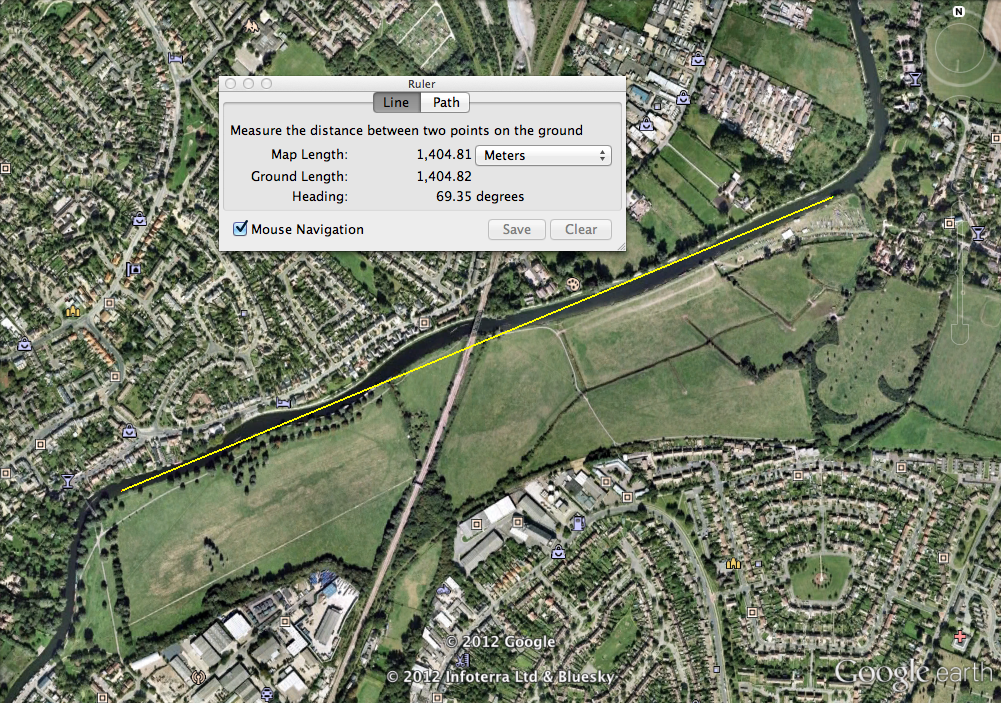
\includegraphics[scale=0.3]{images/TheReach.png}
        \caption{The Reach: roughly 1400m long and straight. By rotating the whole river 20\textdegree \ clockwise can treat it as 70 lots of 20m vectors heading having an angle of 0\textdegree \ from the horizontal (the line apporoximation in Google Earth has a heading of 70\textdegree but this is a bearing so measured clockwise from North unlike standard geometry which measures anti-clockwise from the $x$-axis.)}
        \label{fig:thereach}
      \end{center}
      \end{figure}
      
      Corners were then approximated using sectors a circle, with the river following the arc of the sector. Using Google Earth the radius of the circle of curvature was estimated very approximately. The angle of the sector was approximated by looking at the bearing of line heading into the corner and the bearing of a line heading out of the corner. The angle of the sector was then the difference of these two bearings.
      
      \begin{figure}[h]
      \begin{center}
        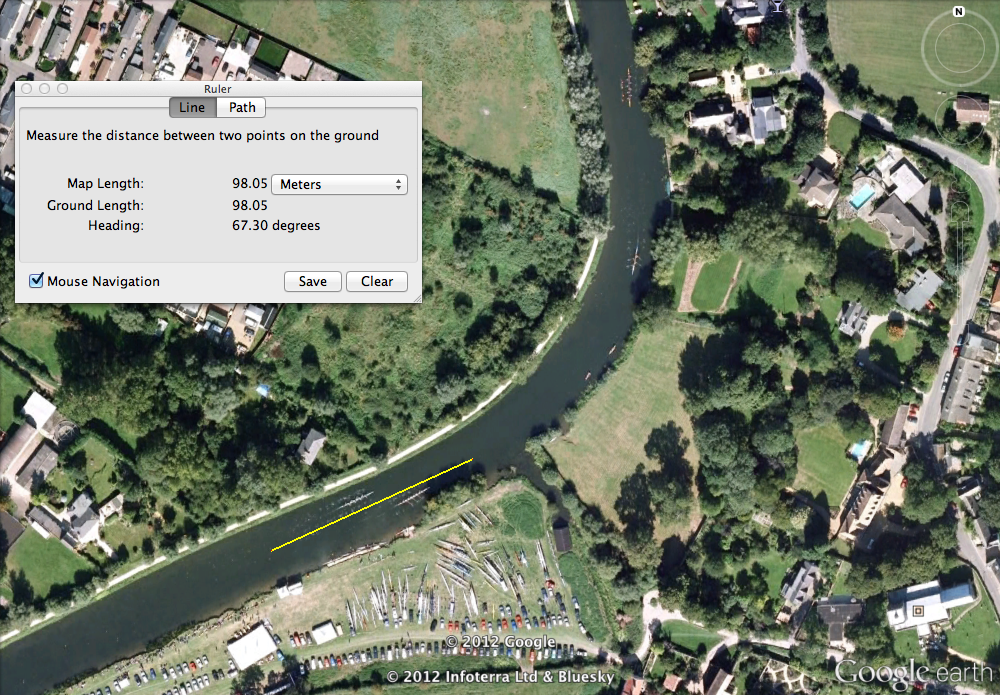
\includegraphics[scale=0.3]{images/DittonCornerHeadingIn.png}
        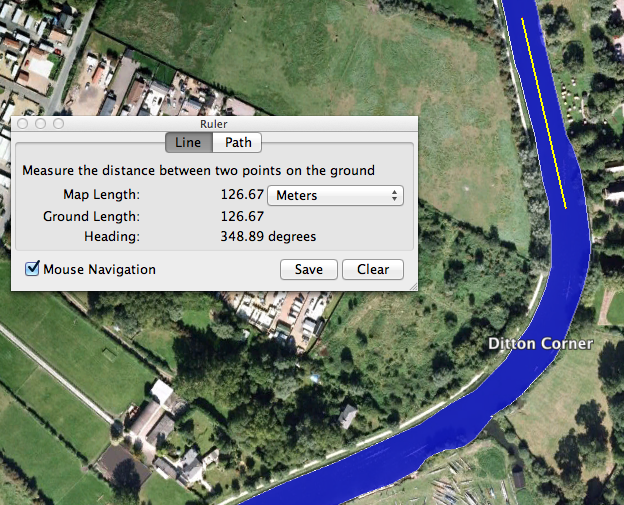
\includegraphics[scale=0.3]{images/DittonCornerHeadingOut.png}
        \caption{Ditton Corner: The heading in is roughly 70\textdegree and the heading out is roughly 170\textdegree so treated this corner as a 90\textdegree sector of a circle (by using a right-angle the calculations were a bit simpler).}
        \label{fig:dittoncorner:angle}
      \end{center}
      \end{figure}
      
      \begin{figure}[h]
      \begin{center}
        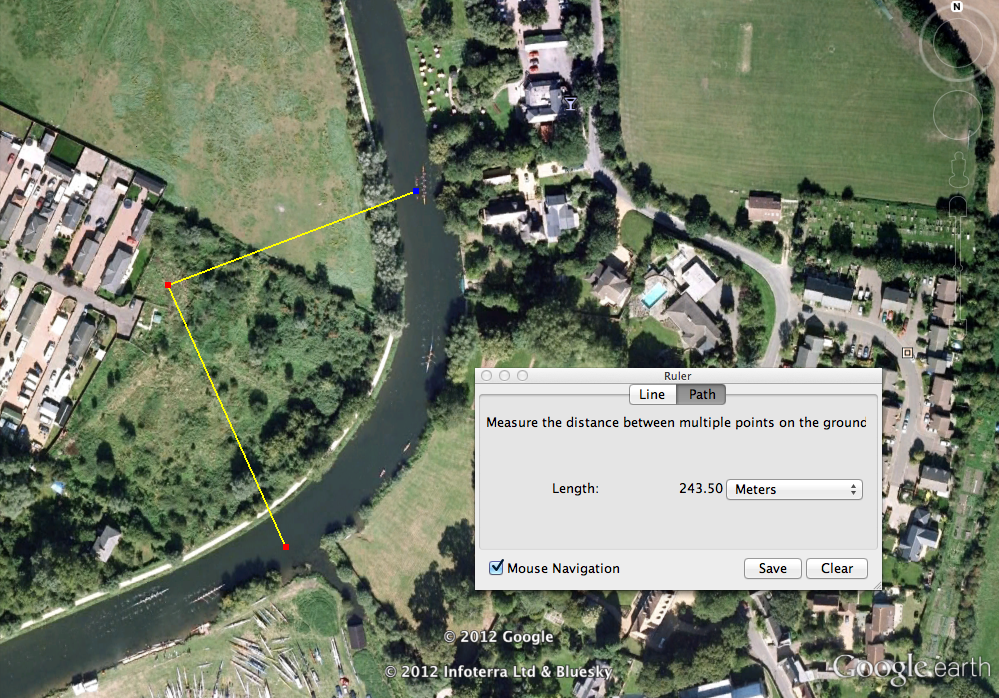
\includegraphics[scale=0.3]{images/DittonCornerRadius.png}
        \caption{Ditton Corner: This shows two approximate radii of the sector that makes up Ditton Corner. Their total length is 244m. Rounded this up and approximated the radius of Ditton Corner to be 125m.}
        \label{fig:dittoncorner:radius}
      \end{center}
      \end{figure}
      
      Figure \ref{fig:dittoncorner:angle} and Figure \ref{fig:dittoncorner:radius} show the values extracted from Google Earth of the heading into and out of a corner (in this case known as Ditton Corner) and an attempt to estimate the radius of the corner. From Figure \ref{fig:dittoncorner:angle}, the heading into the corner is about 70\textdegree and the heading out is about 170\textdegree. Therefore a 90\textdegree sector of a circle would roughly cover this corner. Figure \ref{fig:dittoncorner:radius} shows a rough outline of the radii that make up the sector. The two radii are approximately 250m long, so a single radii would be 125m long. This is for the middle of the river. The radius of the upper lane should be 10m less than this in the 3 lane approximation. And the radius of the lower lane should be 10m more.
      
      Finally for a corner, the arc needed to be approximated by 20m segments. This was done by working out the total length of the arc (radius $\times$ angle) and then dividing by 20. This gave a number of segments. The angle of the first segment was the heading in angle. Each segment's angle was then changed incremented (or decremented depending on whether the river was bending to the left of the right) by (angle of sector)/(number of segments).
      
      In this way the actual path of the river Cam, as can be seen marked out on Google Earth in Figure \ref{techissues:fig:actualcam} is turned into a simplified version as in Figure \ref{techissues:fig:simplecam}.
      
      \begin{figure}[h]
      \begin{center}
        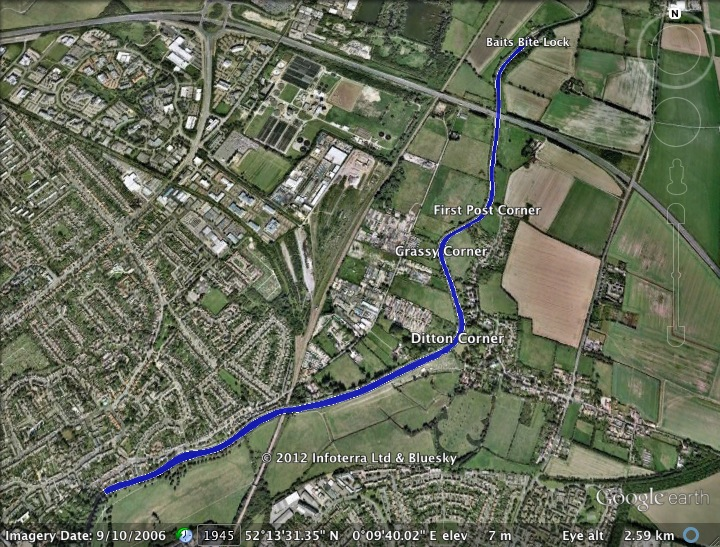
\includegraphics[scale=0.3]{images/GoogleEarthCam.png}
        \caption{The part of the Cam covered by this project marked out on Google Earth. The 3 main corners and Baits Bite Lock have been marked out.}
        \label{techissues:fig:actualcam}
      \end{center}
      \end{figure}
      
      \begin{figure}[h]
      \begin{center}
        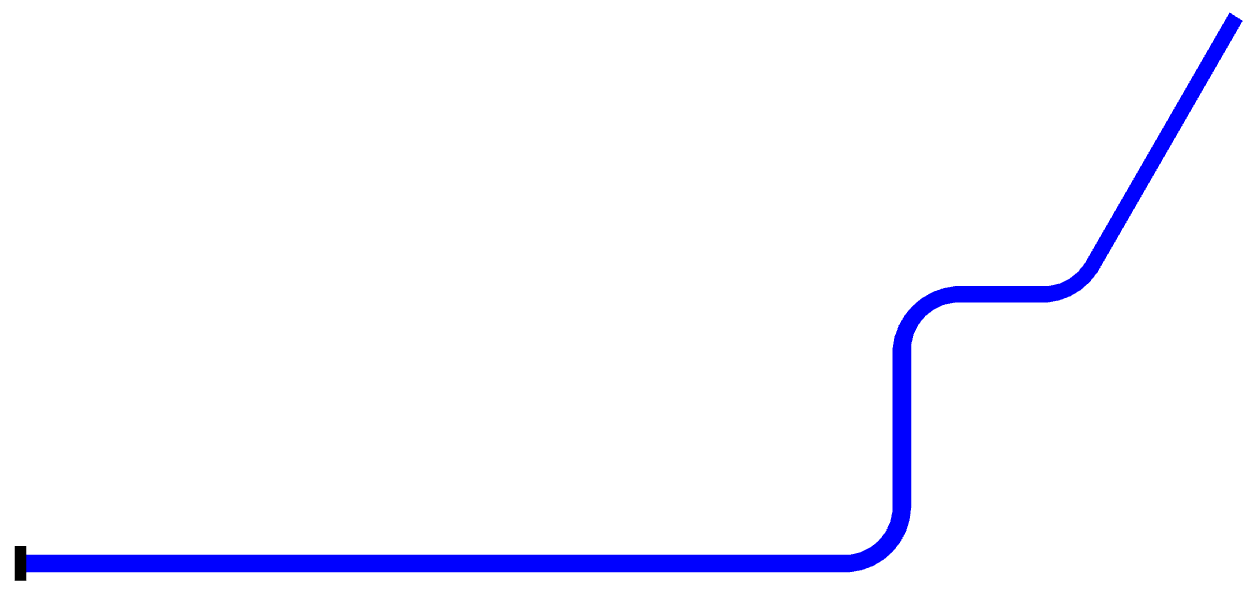
\includegraphics[scale=0.3]{images/SimplifiedCam.png}
        \caption{The simplified version of the Cam as it appears in the visualization. Notice the three corners. The black box represents the boat house.}
        \label{techissues:fig:simplecam}
      \end{center}
      \end{figure}
      
  \section{Action execution}
  The execution of actions by the cox provided two problems. Firstly it was necessary to ensure that if an action was misused (for instance executed in a situation where it did not make sense) then it would not break the system. Secondly boats needed to react to a cox's actions rather than allowing the cox too much direct control over the boat in order to help maintain the indirectness of a cox's control over a boat in the implementation.
  
    \subsection{Ensuring misuse of action does not break system}
    Ideally a cox would not choose to execute an action in a situation where it did not make sense. Unfortunately this is not possible to ensure without artificially limiting a cox's choices. Instead if an action is executed in a non-conforming situation (for example, trying to change lanes when already in the process of changing lanes) the action will revert to a default action. The Let Boat Run action fits nicely with the model as this default action, since it results in the boat continuing forward unchanged. In a way this is equivalent to a cox deciding to carry out an action and then realising it isn't possible.
    
    \subsection{Ordering of cox actions and boat "reaction"}
    \paragraph{Ensuring that the cox cannot influence the boat too directly}
    Scheduled methods on cox and boat objects means that the cox's method can concentrate on the cox's actions. The boat's method will then ensure, whatever the cox decides, that the boat will continue to move forward. In turn, this means that the methods for moving a boat can be shielded from the cox so reduce the risk of a cox's actions influencing the movement of a boat too directly. The one exception to this was the Spin action. For visualization purposes it was necessary to have the boat rotate 180\textdegree while moving in a straight-line across the river, which was very different to the usual boat movement straight forward in the direction the boat was facing. Therefore it was easier for this one off case to have the Spin action call movement methods directly on the boat object. This actually fits nicely with reality where during spinning the cox does tend to control the boat more directly by calling each stroke individually.
      
    \paragraph{Ensuring the boat's movement comes after the cox has execute his action to ensure response}
    Repast has a mechanism for setting the priority of scheduled methods. This means that cox's decision making method can be executed before the boat's movement method and so ensure that the boat's movement will be affected by the cox's decision.
    
    \paragraph{Dealing with actions that take multiple timesteps}
    Some actions by the cox are considered to take multiple time ticks. Spinning is the example. By making each action a class and execution of an action occurring by instantiating an instance of the relevant class and calling the \texttt{execute()} method which returns a boolean to determine whether the action was completed, it was possible to keep a reference to any unfinished actions. These unfinished actions can then be continued at the time tick without the danger of the cox choosing another action which would not make sense. For example, until spinning is complete, it makes no sense to execute any other action.
      
  \section{Time discretization and scale}
    With time broken down into discrete ticks it is necessary to decide what period of time these ticks are supposed to cover. An obvious choice was to make each tick stand for one second. This meant it was possible to store distances as metres and speeds as metres per second in a natural way. Fortunately this choice of tick length also worked well with the visualization as Repast offered a way to put delays between the ticks so that a simulation can either be run very quickly through to it being possible to watch it in an equivalent to real time. This tick length also meant a boat would move a relatively short distance each tick so movement appears smooth and there is less danger of getting into unusual situations of boats jumping long distances.
    
  \section{Visualization}
    It was important for this project to have a visualization. Most importantly the visualization allows anyone to observe the effects of particular control policies. It is easy to spot where bottlenecks in traffic flow might be occurring and occasionally the cause (perhaps by not allowing boats to overtake, a single slow boat holds up everyone? perhaps by allowing boats to crash into each other, a large pile up occurs at the lock where boats take a long time to spin). A visualization was also a useful tool for debugging the simulation and ensuring that the boats where behaving as expected. Fortunately Repast provides a API to visualize the changes to objects each tick - in this case to show where the boats have moved to on the river each tick.
    
    The visualization has two main elements. The static river and the moving boats. Drawing the river provided a large challenge covered in its own section (see Section \ref{techissues:river}). Drawing the boats was not without problems despite how easy Repast makes it to show objects moving around a continuous 2D space Originally the boats where all red rectangles. This made them very simple to draw. However these rectangles were not particularly intuitive to look at and they presented two problems:
    \begin{enumerate}
      \item \label{techissues:visualization:boat_shape} It was not possible to tell which way boat was pointing.
      \item \label{techissues:visualization:boat_colour} The boats could be hard to tell apart from each other since they were the same colour. 
    \end{enumerate}
    As with the river, problem \ref{techissues:visualization:boat_shape} was solved using Java's Path2D API to draw a more appropriate shape with 8 oars and a pointed bow to point forwards. Problem \ref{techissues:visualization:boat_colour} was solved by giving each boat a randomly selected colour. These can be seen in Figure \ref{techissues:fig:boats}.
    
    \begin{figure}[h]
    \begin{center}
      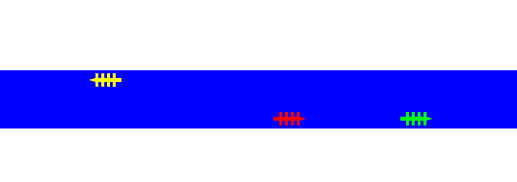
\includegraphics[scale=0.3]{images/boats.png}
      \caption{Multi-coloured boats: notice the shape of the boat with 8 spines to represent the 8 oars. The front of the boat points forward, while the back is flat.}
      \label{techissues:fig:boats}
    \end{center}
    \end{figure}
      
  \section{Experiment Framework}
  In order to evaluate the control policies it was necessary to run experiments and collect data. There are two phases to the experiments. First an experiment needs to be setup which includes scheduling boats to be launched and their launch parameters. Secondly while the experiment runs data needs to be collected about the boats such as how many times they crash and how many ticks it takes for each to complete their outing and return to the boat house. Both these were achieved using a MySQL database although Repast does have both a batch run environment where many simulations can be run with varying parameters and a mechanism to collect data during a simulation run. Storing data for setting up and experiment and data collected during an experiment in a database meant it was easy to organise the data and ensure it persisted so the same experiment could be run multiple times and their results compared. As each experiment requires parameters for each boat launched, a database provided an easier way to organise lots schedules with lots of launches compared to setting many parameters (each launch has 5 parameters and a schedule has tens of launches) in a batch run. Repast's data collection only allowed outputting the data to a file. Although Repast offered file formats such as csv, a database offered a much easier way to create a structured, permanent record of experimental data for later analysis.
  
  \subsection{Experiment Setup}
  Each experiment corresponds to a row in the database with fields for storing the random seed, the control policy the coxes should follow and the schedule to follow. A schedule consists of a set of boat launches to schedule along with the parameters to use. These parameters are the minimum distance the boat should cover in the outing (which for this project was constant at 5000m, roughly equivalent to a run to the lock and back), the speed multiplier (again for this project a constant at 0.5, which meant a boat in gear 10 would travel at 5m/s which roughly matches the 6.3m/s of the world record over 2km), the gear the boat would ideally travel in and the tick the boat should be launched at. 
  
  Experiments and launch schedules based on parameters such as number of boats to launch and delay between each launch can be created using simple scripts. The creation of schedules is completely independent to running the simulation. All that matters is the data ends up in the database. This meant it was easy to write the scripts using Ruby. The ease-of-use of the Ruby language and the object relational mapper (ORM) Active Record made it very quick to write these scripts which can quickly create new schedules. This was much simpler than using a Java ORM like Hibernate which requires lots of configuration.
  
  When each simulation begins it checks a parameter called Experiment Id and looks up the row in the database corresponding to this experiment id. It then looks up the scheduled launches associated with this experiments and schedules the \texttt{launch()} method to run on the boathouse object with the launch parameters set in the database at the appropriate ticks.
  
  \subsection{Data Collection}
  While an experiment runs, data collected is stored in the database. A record of the parameters used at each stage (like the random seed and launch tick of each boat) is stored. Therefore if an experiment or schedule is edited there is still an accurate record of what happened. Plus new data is generated such as how far the boat actually moved and the number of crashes that occurred. Repast allows the scheduling of methods to run at the end of a simulation run. One was setup to flush all the data collected to the database. Since this occurs in the simulation, JDBC is used to connect to the database in Java. Although this requires a bit more work writing SQL queries compared to Ruby and ActiveRecord, since the simulation was creating the data the process of adding the data to the database was not as complicated as generating schedules and so it was not a large problem.
  
  Methods were added to the simulation to generate the data.
  \begin{itemize}
    \item Each time a crash occurs the crash counter of the in progress experiment is incremented.
    \item At the end of a boat's scheduled \texttt{run()} method is a call to a method which updates that boat's records with information like how far the boat had now moved in total.
    \item When a boat landed, it's record would be flushed to the database to reduce the amount of data that had to be flushed at the end and to ensure that some data is in the database in case something went wrong later in the simulation.
  \end{itemize}
  
  In this way it is straight-forward to set up new experiments and keep a permanent record of any data collected during the experiment.

